% ===========================================================================
%  Beamer slides: In-plane orthotropic elastic wave control by fiber design
%  Build:  TEXMFVAR=/home/jrt/wavetopo/.texcache pdflatex slides.tex   (x2)
% ===========================================================================
\documentclass[aspectratio=169,10pt]{beamer}

\usetheme{metropolis}
\usepackage{amsmath}                      % MUST precede newtxmath
\usepackage{amsthm}

% ---- fonts -------------------------------------------------------------- %
% The newtx pairing, loaded plainly and unconditionally.  If it is missing you
% get an explicit "File newtxtext.sty not found" and can install it -- which is
% far better than a silent fallback that merely looks like standard LaTeX.
%
% Constraints this satisfies:
%   * amsmath and amsthm are loaded BEFORE newtxmath (top of file); amsthm in
%     particular, or \openbox ends up defined twice
%   * amssymb is NOT loaded -- newtxmath supplies the AMS symbols itself, and
%     loading both errors on \square, \lesssim, \gtrsim, \mathbb
%   * \usepackage{times} is obsolete and would give Times text with Computer
%     Modern maths -- exactly the half-applied pairing to avoid; removed
%   * bm and mathalfa must follow the math font
\usepackage{newtxtext,newtxmath}
\usepackage{bm}
\usepackage{booktabs}
\usepackage{graphicx}
\usepackage{tikz}
\usetikzlibrary{arrows.meta,positioning,calc}

\graphicspath{{figs/}}

% ---- notation --------------------------------------------------------- %
% NOTE: these are defined with \providecommand+\renewcommand, NOT \newcommand.
% Short names like \T, \HH, \ii and \Real are defined by some packages/engines
% (\T is a text accent in several).  With \newcommand a pre-existing definition
% makes the declaration FAIL while silently keeping the old meaning, and every
% later use in math mode then raises "Missing $ inserted" far from the cause --
% a failure that appears on MiKTeX but not on TeX Live, or vice versa.
% \providecommand+\renewcommand always installs our meaning.
\makeatletter
\newcommand{\DefN}[2]{\@ifundefined{\expandafter\@gobble\string#1}{}{%
    \PackageInfo{notation}{overriding pre-existing \string#1}}%
  \providecommand#1{}\renewcommand#1{#2}}
\makeatother
\DefN{\vth}{\bm{\theta}}
\DefN{\vu}{\mathbf{u}}
\DefN{\vx}{\mathbf{x}}
\DefN{\vU}{\mathsf{U}}
\DefN{\vb}{\mathsf{b}}
\DefN{\veps}{\bm{\varepsilon}}
\DefN{\ii}{\mathrm{i}}
\DefN{\T}{^{\mathsf{T}}}
\DefN{\HH}{^{\mathsf{H}}}

% numbers shared with the paper (needs \DefN above)
% Shared result numbers: \input by BOTH the paper and the slides so a
% number can never be updated in one and stale in the other.
% curl-constraint result numbers (set from examples/dolfinx_lens.py curl)
\newcommand{\CURLU}{6.3}
\newcommand{\CURLC}{2.8}
\newcommand{\GAINU}{47}
\newcommand{\GAINC}{12}
% through-hole lens numbers (examples/dolfinx_lens.py hole)  -- TO FILL
\newcommand{\HGAINU}{49}
\newcommand{\HCURLU}{5.7}
\newcommand{\HGAINC}{17}
\newcommand{\HCURLC}{3.55}
\newcommand{\HRINV}{3.57}
% through-hole cloak numbers (examples/dolfinx_cloak_soft.py curl) -- TO FILL
\newcommand{\CKREDU}{31}
\newcommand{\CKCURLU}{3.4}
\newcommand{\CKREDC}{21}
\newcommand{\CKCURLC}{1.7}
\newcommand{\CKZALL}{1.72}
% asymmetric through-hole lens (examples/dolfinx_lens.py holeasym) -- TO FILL
\newcommand{\AGAIN}{50}
\newcommand{\ACURL}{4.24}
\newcommand{\ALIM}{4.17}
% curved energy routing / joint protection (examples/dolfinx_guide_joint.py)
\newcommand{\GEXIT}{698}    % exit-port energy gain
\newcommand{\GGUARD}{0.17}   % guard-annulus energy ratio (<1 is good)
\newcommand{\GPROT}{4002}    % protection factor (exit/guard ratio improvement)
\newcommand{\GRATZ}{127}    % baseline guard/exit ratio
\newcommand{\GZ}{6.59}       % max|zeta| of the reported design
\newcommand{\GZALL}{6.67}  % 1/R_TOW (print head), NOT 1/R_J
\newcommand{\GCONFZ}{22}   % downstream confinement, baseline
\newcommand{\GCONFO}{97}   % downstream confinement, optimized
% multi-target beam shaping (examples/dolfinx_lens.py multi) -- TO FILL
\newcommand{\MCONA}{2}
\newcommand{\MCONB}{19}
\newcommand{\MTGAIN}{19}
\newcommand{\MCIMP}{10}
% flat-band metamaterial (examples/flatband_demo.py) -- TO FILL
\newcommand{\FBBAND}{3}
\newcommand{\FBWZ}{2.78}
\newcommand{\FBWO}{0.59}
\newcommand{\FBFLAT}{4.7}
\newcommand{\FBGU}{+0.42}
\newcommand{\FBGD}{+0.66}
\newcommand{\FBWV}{0.65}
\newcommand{\FBGUV}{+0.41}
\newcommand{\FBGDV}{+0.67}


\title{In-Plane Orthotropic Elastic Wave Control\\by Fiber-Orientation Design}
\subtitle{model, adjoint, algorithms, results}
\date{\today}
\author{}

\begin{document}
\maketitle

% ======================================================================== %
\begin{frame}{The question}
\begin{columns}[T]
\begin{column}{0.56\textwidth}
Can we steer elastic waves in a composite plate by designing \emph{only} the
local fiber orientation $\theta(\vx)$ --- no topology, one material?
\medskip

\textbf{Why it might work.} A continuous-fiber composite is strongly orthotropic:
\[
  E_{f1}/E_{f2}\approx 15 \;\Longrightarrow\; c_{\rm fast}/c_{\rm slow}\approx 3.8
\]
\medskip

\textbf{Why it might not.} Orientation is a single scalar per point, and the wave
equation is only weakly coupled to it \dots\ unless the material is anisotropic.
\end{column}
\begin{column}{0.42\textwidth}
\begin{block}{The lever, precisely}
\[
  \mathbf D_f(\theta)=\mathbf T(\theta)\,\mathbf Q_f\,\mathbf T(\theta)\T
\]
\[
  \mathbf Q_f\ \text{isotropic}\iff
  \frac{\partial\mathbf D_f}{\partial\theta}\equiv\bm 0
\]
Every gradient in this work is built from
$\partial\mathbf D_f/\partial\theta$, so for an isotropic plate the design
sensitivity is \emph{identically zero}.
\end{block}
\end{column}
\end{columns}
\end{frame}

% ======================================================================== %
\section{Model}

\begin{frame}{Time-harmonic in-plane elastodynamics}
Plane stress, $\vu(\vx)e^{-\ii\omega t}$, rotated orthotropic stiffness:
\[
  \bigl[(1+\ii\eta)\mathbf K(\vth)-\omega^2\mathbf M+\ii\omega\mathbf C\bigr]\vu=\mathbf f
\]
\begin{itemize}
  \item $\mathbf K$ from $\mathbf D_f(\theta)$ --- the only $\theta$-dependent operator
  \item $\eta$: structural (hysteretic) damping; $\mathbf C$: quadratic absorbing sponge
  \item genuine \emph{vector} physics, not a reduced antiplane scalar model
\end{itemize}
\vfill
\begin{alertblock}{The installed PETSc is a \emph{real} build}
So the complex system is solved by an exact real four-field split --- and the
split has to be provably lossless, not merely convenient.
\end{alertblock}
\end{frame}

\begin{frame}{The real four-field split}
With $A=\mathbf K-\omega^2\mathbf M$ and $B=\eta\mathbf K+\omega\mathbf C$ (both real symmetric),
\[
  (A+\ii B)(\vu_r+\ii\vu_i)=\mathbf f
  \;\Longleftrightarrow\;
  \underbrace{\begin{bmatrix} A & -B\\ B & \phantom{-}A\end{bmatrix}}_{\mathcal A}
  \begin{bmatrix}\vu_r\\ \vu_i\end{bmatrix}
  =\begin{bmatrix}\mathbf f_r\\ \mathbf f_i\end{bmatrix}
\]
\begin{block}{Two facts that make this free}
\begin{enumerate}
  \item Equating real and imaginary parts is exact ($\{1,\ii\}$ is a basis of
        $\mathbb C$ over $\mathbb R$) --- nothing is approximated.
  \item $\mathcal A\T$ is the realification of $(A+\ii B)\HH$. \\
        \textbf{So the transposed \emph{real} solve returns the true complex
        adjoint.}
\end{enumerate}
\end{block}
\emph{Cost:} $\sim2\times$ a native complex LU. With complex \texttt{PETSc} the
whole construction collapses to one line, and no reported number changes.
\end{frame}

\begin{frame}{Discrete spaces}
\centering\small
\begin{tabular}{lll}
\toprule
& wave control (\texttt{dolfinx}) & periodic cell (Q4, \texttt{numpy/scipy})\\
\midrule
cells       & triangles ($\mathbb P_1$)      & rectangles (Q4 bilinear)\\
state       & $[\mathbb P_1]^4$, 4 dof/node  & Q4 vector, 2 dof/node\\
            & $(u^r_x,u^r_y,u^i_x,u^i_y)$    & $(u_x,u_y)$\\
design      & $\mathbb{DG}_0$ per cell       & element-wise constant\\
solve       & sparse LU (MUMPS)              & dense Hermitian \texttt{eigh}\\
dual        & adjoint in the same space, $\mathcal A\T$ & eigenvalue perturbation\\
\bottomrule
\end{tabular}
\vfill
\begin{itemize}
  \item Holes are \emph{cut from the geometry} (conforming \texttt{gmsh}), not
        soft SIMP voids --- a staircased rim scatters on its own account and
        blurs the very radius the curvature rule is tied to.
  \item Two independent codes share the physics and the design machinery, but
        no assembly or linear algebra: each is a check on the other.
\end{itemize}
\end{frame}

% ======================================================================== %
\section{Sensitivity and algorithms}

\begin{frame}{Discrete adjoint in two lines of UFL}
Adjoin $\mathcal A(\vth)\vU=\vb$ with $\bm\Lambda$; kill the implicit state term:
\[
  \boxed{\ \mathcal A\T\bm\Lambda=-\partial J/\partial\vU\ }
  \qquad
  \boxed{\ \frac{\mathrm dJ}{\mathrm d\theta_\ell}=\frac{\partial R}{\partial\theta_\ell}\ }
\]
\[
  \frac{\mathrm dJ}{\mathrm d\theta_\ell}
  =\int_{\Omega_\ell}\Bigl[\veps(\vu_r)\T\tfrac{\partial\mathbf D_f}{\partial\theta}\veps(\bm\lambda_r)
  +\veps(\vu_i)\T\tfrac{\partial\mathbf D_f}{\partial\theta}\veps(\bm\lambda_i)+\dots\Bigr]
\]
\begin{itemize}
  \item mass, sponge and source carry no $\theta$: they drop out
  \item the whole gradient is built from $\partial\mathbf D_f/\partial\theta$
        --- hence the isotropy result is exact, not asymptotic
  \item FD-verified to $\sim\!10^{-6}$; one LU reused for forward \emph{and} adjoint
\end{itemize}
\end{frame}

\begin{frame}{Two gradient chains}
\textbf{Chain A --- orientation-only wave control}
\[
  \hat\theta\xrightarrow{\ \mathbf S\ }\hat\theta^{\rm sym}
  \xrightarrow{\ \mathbf B\ }\theta
  \xrightarrow{\mathbf D_f}\mathcal A
  \xrightarrow{\rm solve}\vU\longrightarrow J
\]
\[
  \nabla_{\hat\theta}\bigl[-\ln E+\mu\Pi\bigr]
  =-\tfrac{1}{E}\,\mathbf S\T\mathbf B\T\mathbf d
  +\mu\,\mathbf S\T(\partial\bm\zeta/\partial\hat\theta)\T\mathbf q
\]
\medskip
\textbf{Chain B --- two-field Bloch co-design}
\[
  z\xrightarrow{\ \mathbf P\ }\tilde y\xrightarrow{\ \mathbf E_{\mathcal F}\ }y
  \xrightarrow{\rm SIMP}\mathbf K,\mathbf M,
  \qquad
  \hat\theta\xrightarrow{\ \mathbf B\ }\theta
\]
\[
  \nabla_zJ=\mathbf P\T\mathbf E_{\mathcal F}\Bigl[\partial J/\partial y+2c_v(\bar z-v^\star)\mathbf A/\textstyle\sum_jA_j\Bigr]
\]
\vfill
Every operator contributes exactly one transposed factor. $\mathbf S$ is an
orthogonal projector, so symmetrizing the design and the gradient are the
\emph{same} operation.
\end{frame}

\begin{frame}{Manufacturing enters the optimization, not the post-processing}
\begin{columns}[T]
\begin{column}{0.5\textwidth}
\textbf{CS-RBF orientation}\\
$\theta=\mathbf B\hat\theta$, Wendland $C^2$, row-stochastic
\medskip

\textbf{Fiber curvature}
\[
  \zeta=(\mathbf n\!\cdot\!\nabla)\theta,\qquad |\zeta|\le\zeta_{\rm all}
\]
$\zeta_{\rm all}=1/R$ for a hole the tows must wrap;
$1/R_{\rm tow}$ for a steered channel --- \emph{these are different constraints}.
\end{column}
\begin{column}{0.5\textwidth}
\textbf{Toolpaths by wave projection}
\[
  \nabla\psi=[-\sin\theta,\cos\theta]\T,\quad
  \chi=\tfrac12+\tfrac12\cos(2\pi\psi/d)
\]
Solved as a least-squares gradient match --- the normal-equations Poisson form
drops the boundary flux and collapses the pitch.
\medskip

On a periodic cell: FFT Helmholtz projection $+$ an \emph{integer} number of tow
cycles, so tows join across every boundary.
\end{column}
\end{columns}
\end{frame}

\begin{frame}{Data flow}
\centering
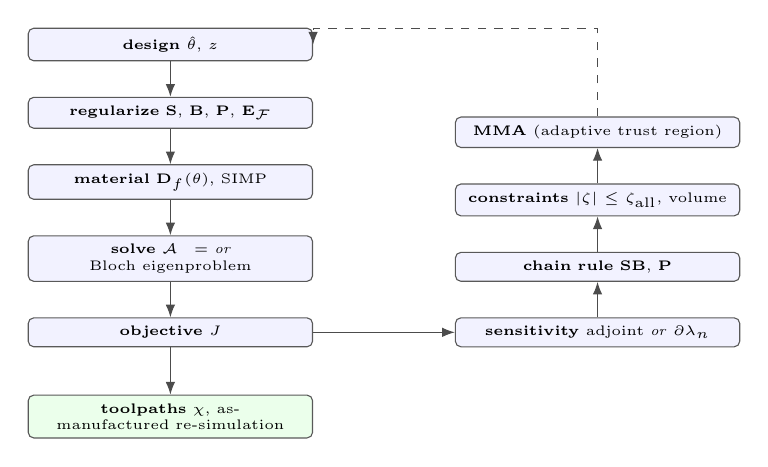
\begin{tikzpicture}[node distance=4.5mm and 10mm,
  blk/.style={rectangle,rounded corners=2pt,draw=black!65,fill=blue!5,
              align=center,inner sep=3pt,font=\tiny,text width=34mm},
  ar/.style={-{Latex[length=1.6mm]},draw=black!70}]
\node[blk] (d) {\textbf{design} $\hat\theta$, $z$};
\node[blk,below=of d] (r) {\textbf{regularize} $\mathbf S$, $\mathbf B$, $\mathbf P$, $\mathbf E_{\mathcal F}$};
\node[blk,below=of r] (m) {\textbf{material} $\mathbf D_f(\theta)$, SIMP};
\node[blk,below=of m] (s) {\textbf{solve} $\mathcal A\vU=\vb$ \emph{or} Bloch eigenproblem};
\node[blk,below=of s] (j) {\textbf{objective} $J$};
\node[blk,right=18mm of j] (g) {\textbf{sensitivity} adjoint \emph{or} $\partial\lambda_n$};
\node[blk,above=of g] (c) {\textbf{chain rule} $\mathbf S\T\mathbf B\T$, $\mathbf P\T$};
\node[blk,above=of c] (k) {\textbf{constraints} $|\zeta|\le\zeta_{\rm all}$, volume};
\node[blk,above=of k] (u) {\textbf{MMA} (adaptive trust region)};
\node[blk,below=6mm of j,fill=green!8] (t) {\textbf{toolpaths} $\chi$, as-manufactured re-simulation};
\draw[ar](d)--(r); \draw[ar](r)--(m); \draw[ar](m)--(s); \draw[ar](s)--(j);
\draw[ar](j)--(g); \draw[ar](g)--(c); \draw[ar](c)--(k); \draw[ar](k)--(u);
\draw[ar,dashed](u.north)|-($(d.east)+(0,2mm)$)--(d.east);
\draw[ar](j)--(t);
\end{tikzpicture}
\end{frame}

% ======================================================================== %
\section{Results}

\begin{frame}{Curvilinear-fiber wave lens}
\centering
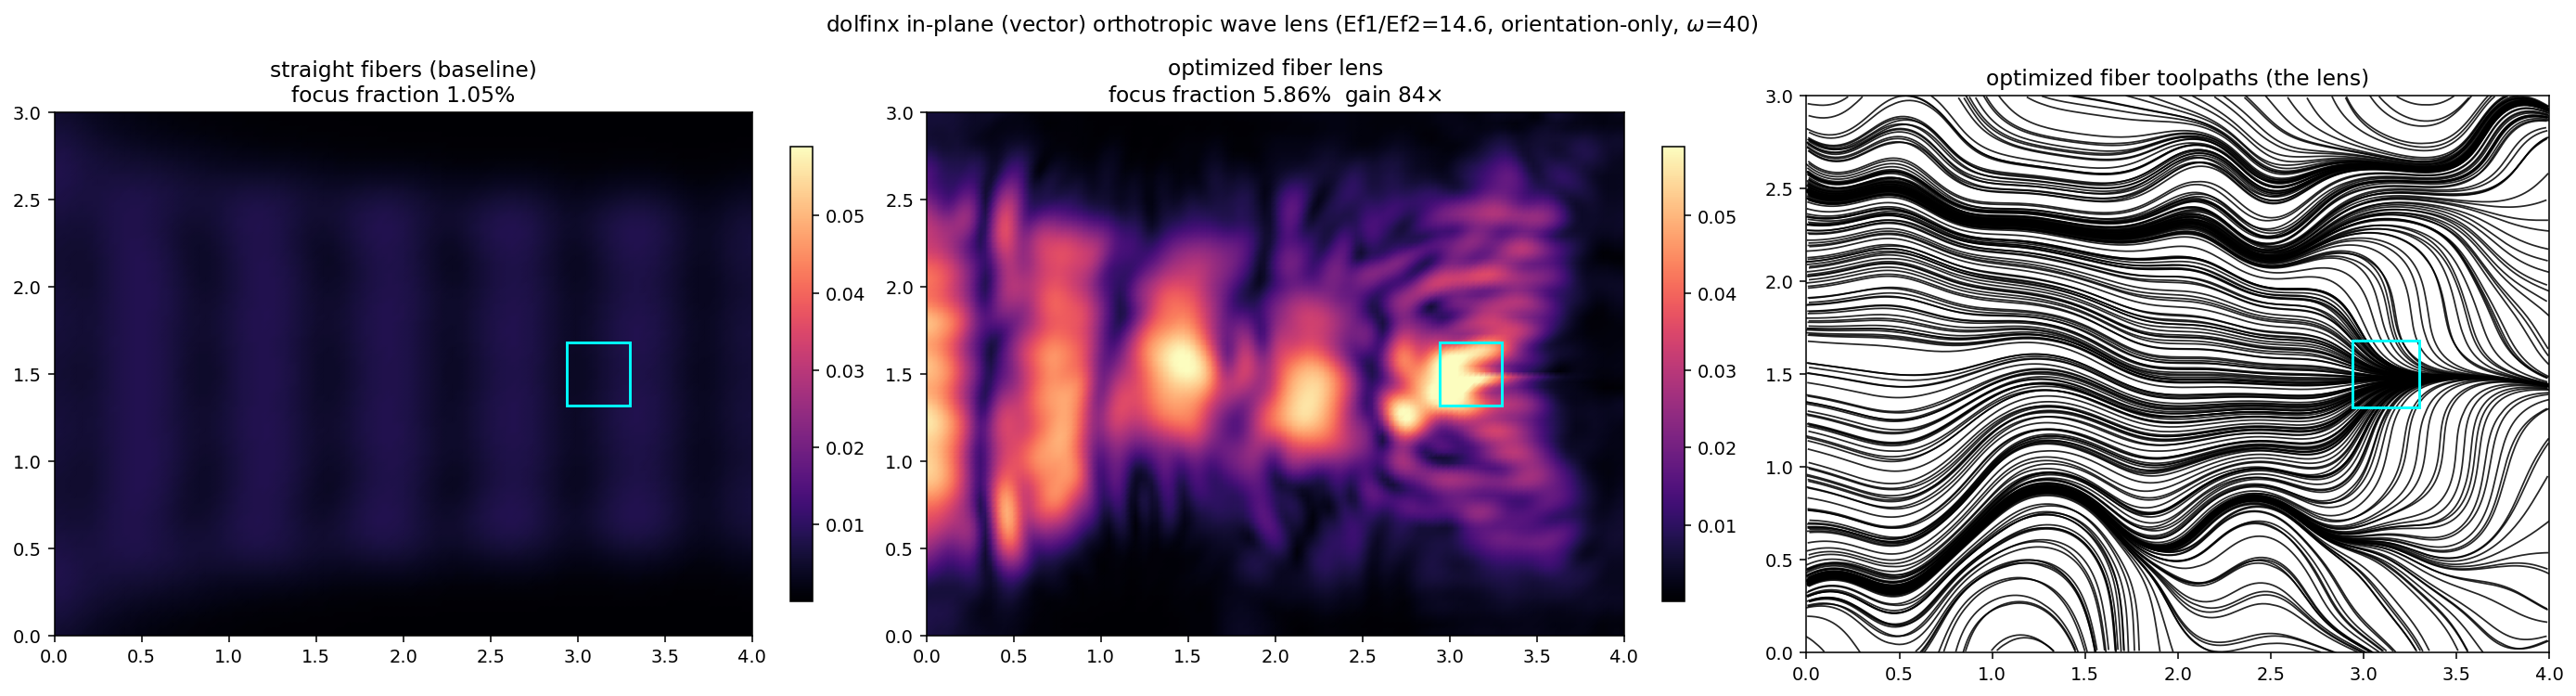
\includegraphics[width=0.82\textwidth]{dfx_lens.png}\\
\small Orientation-only design: $\mathbf{78\times}$ focus-energy gain, focus
fraction $1.05\%\to7.68\%$. Mirror symmetry imposed by the projector $\mathbf S$.
\end{frame}

\begin{frame}{Manufacturability costs performance --- honestly}
\centering
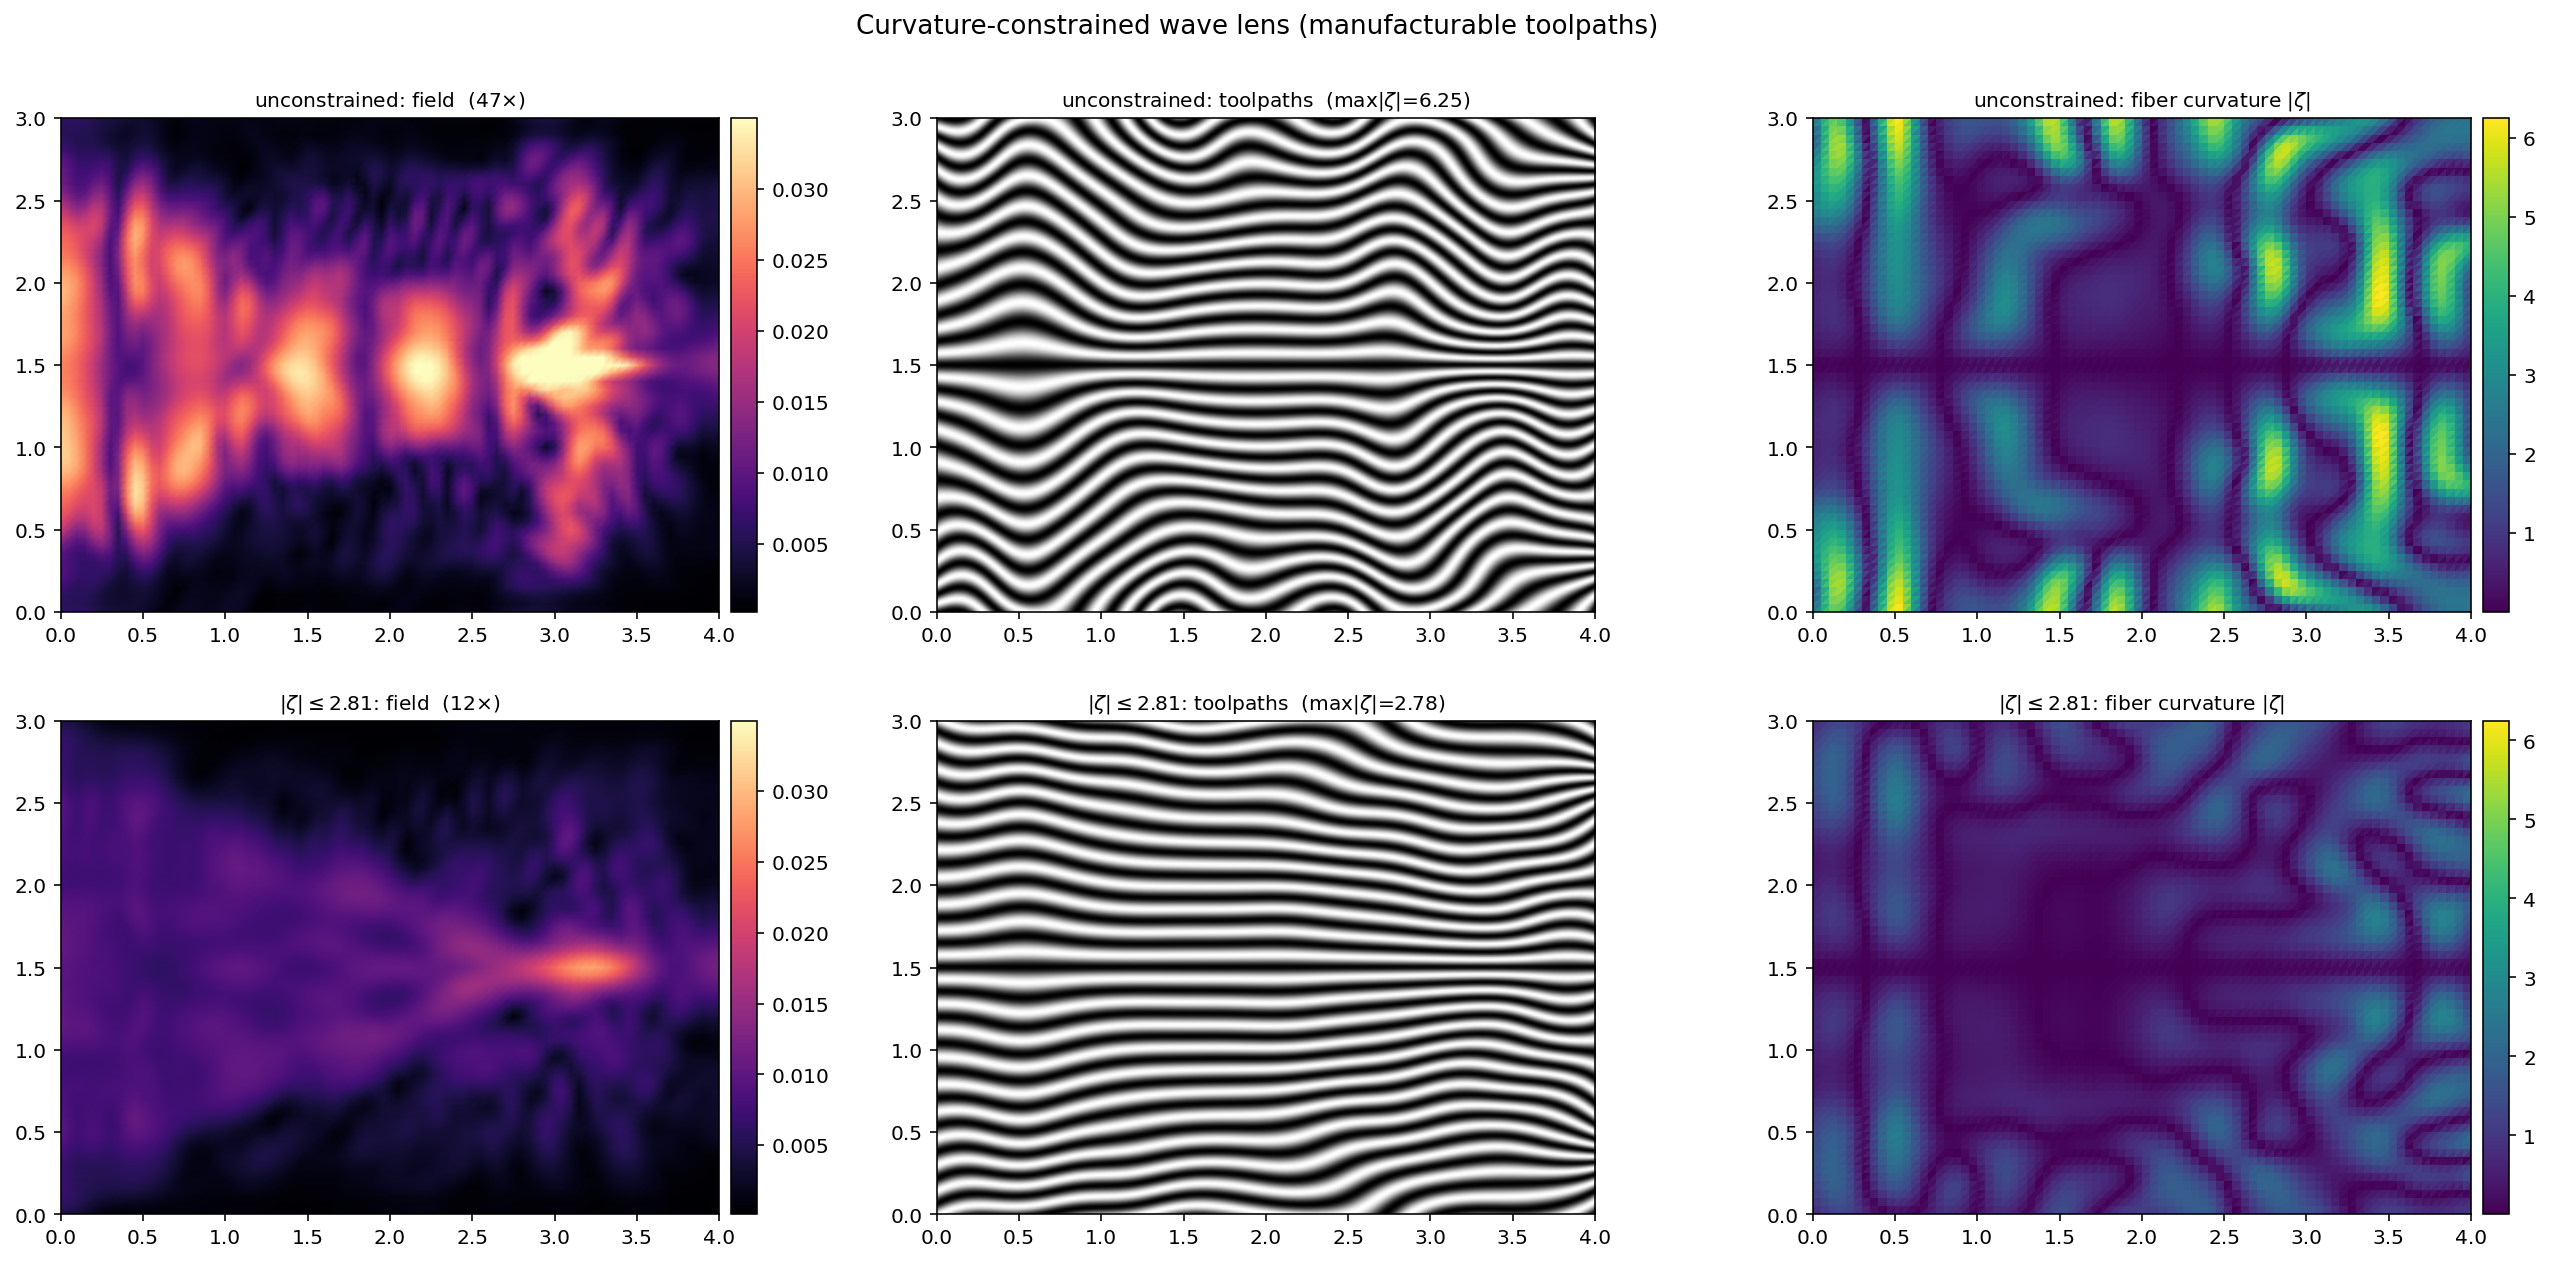
\includegraphics[width=0.80\textwidth]{dfx_lens_curl.png}\\
\small Bounding $|\zeta|\le\CURLC$ relaxes the tight bends and the gain falls
$\GAINU\times\!\to\!\GAINC\times$. This trade-off is the point, not a defect.
\end{frame}

\begin{frame}{Designing around prescribed through-holes}
\centering
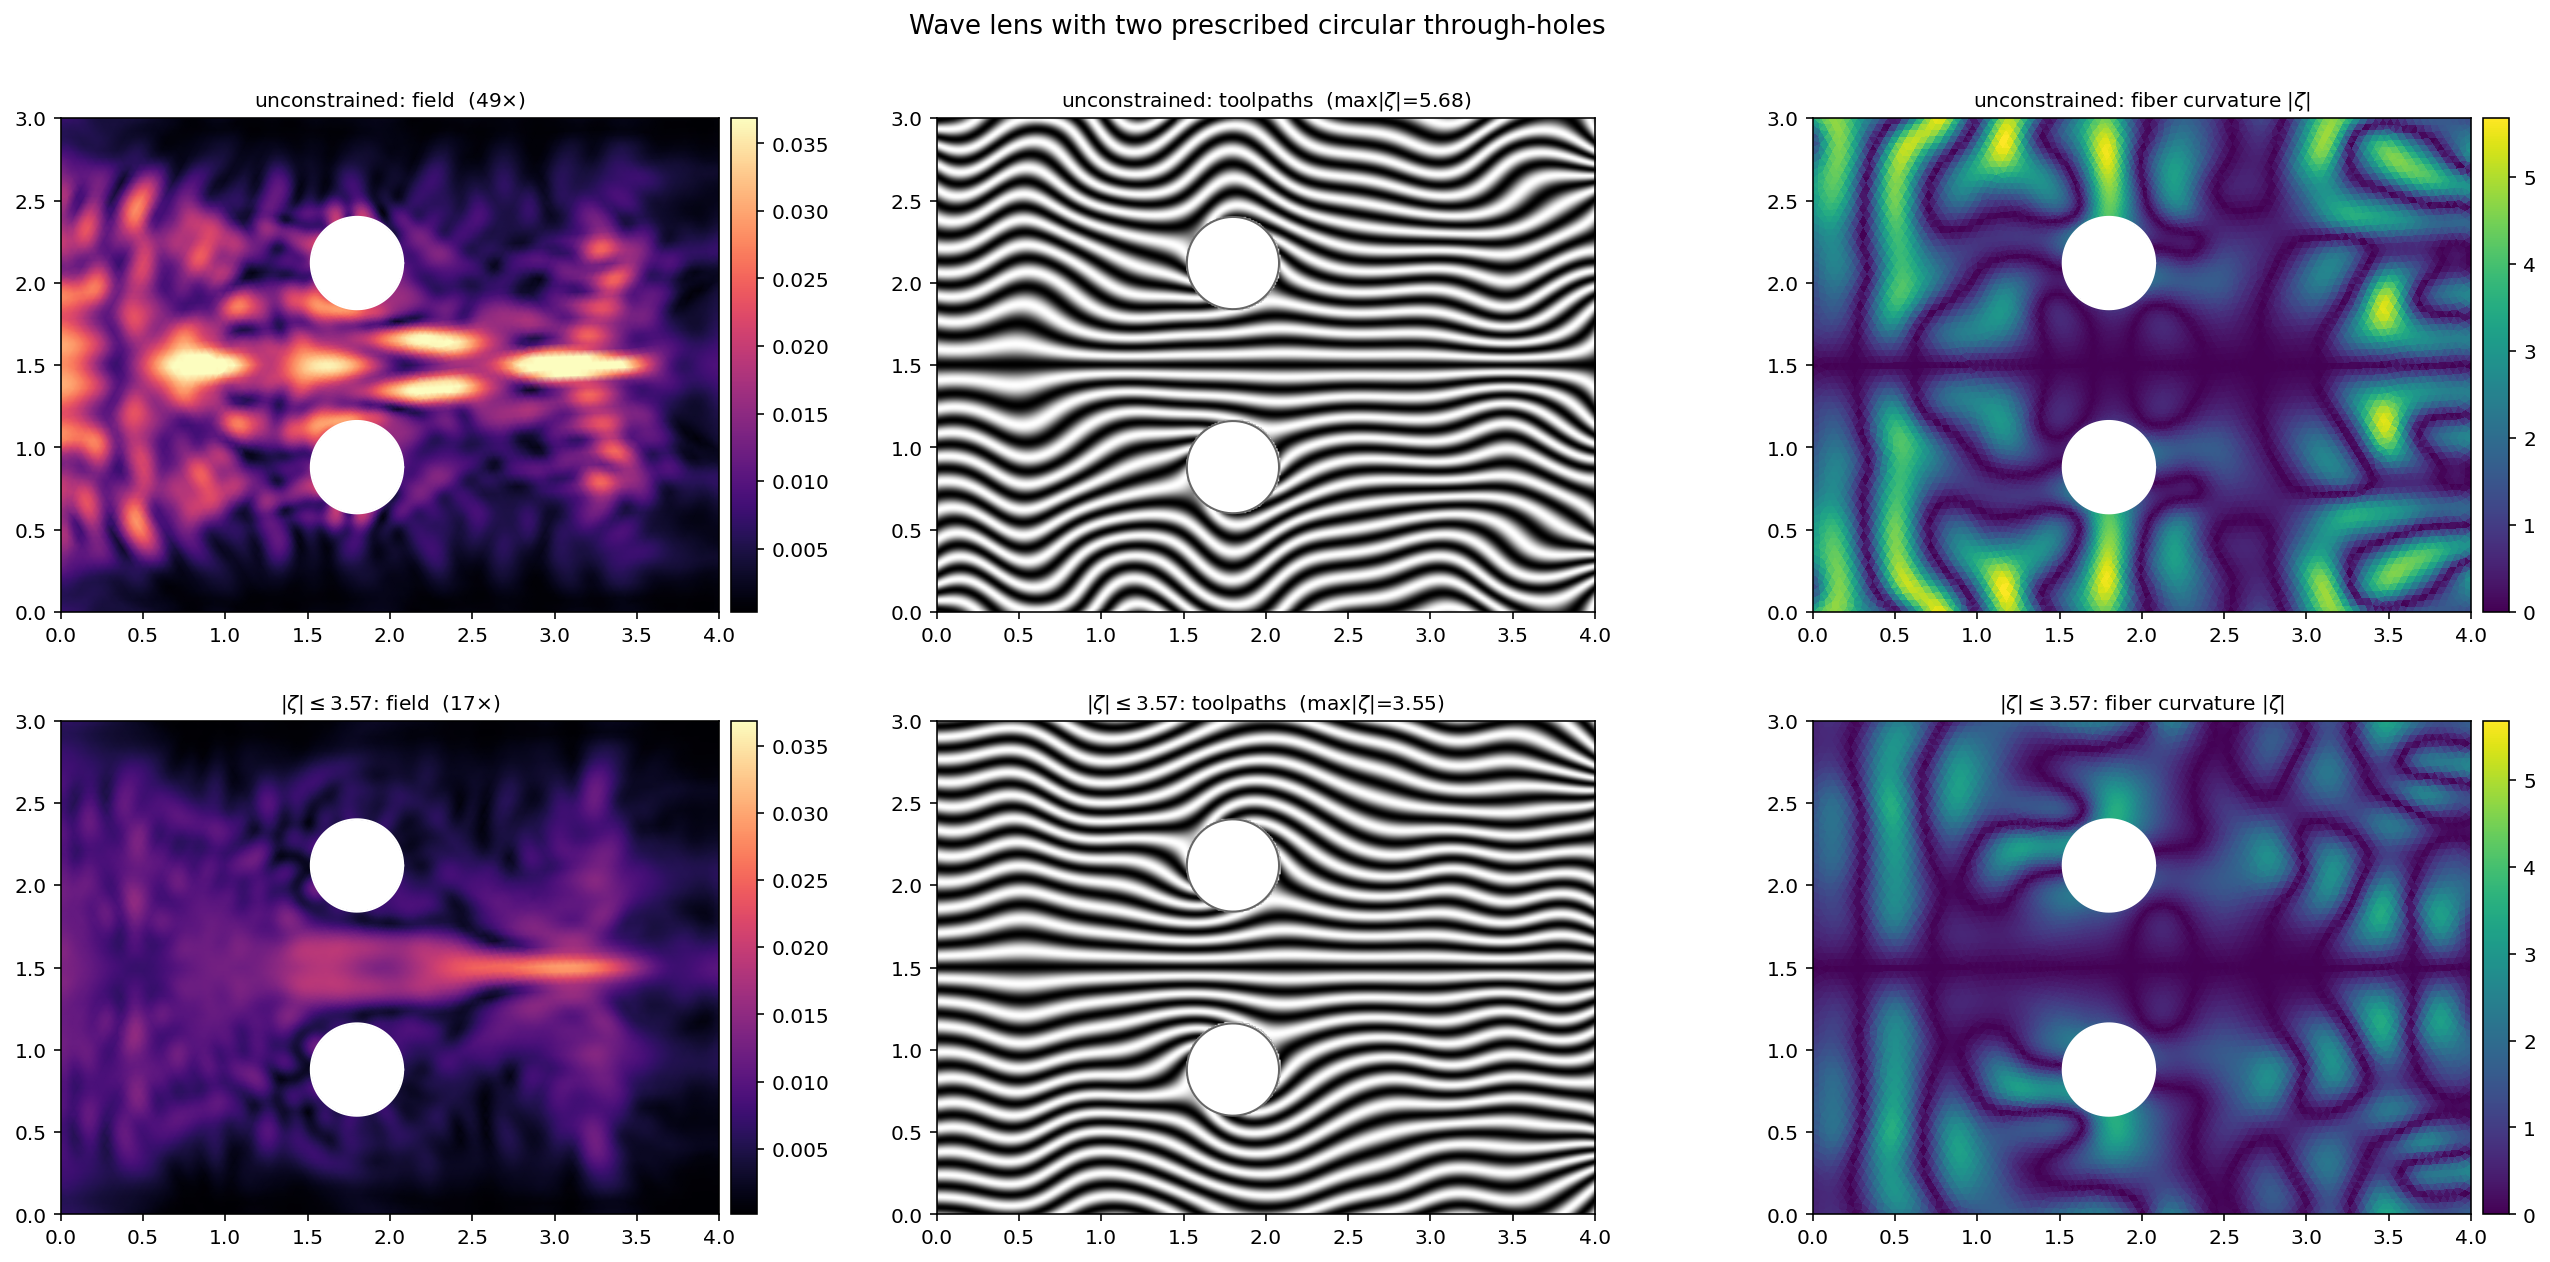
\includegraphics[width=0.78\textwidth]{dfx_lens_hole.png}\\
\small Holes \emph{cut from the geometry}: $\HGAINU\times$ unconstrained,
$\HGAINC\times$ under $|\zeta|\le1/R=\HRINV$ (feasible: $\HCURLC<\HRINV$).
\end{frame}

\begin{frame}{The design is re-solved per geometry}
\centering
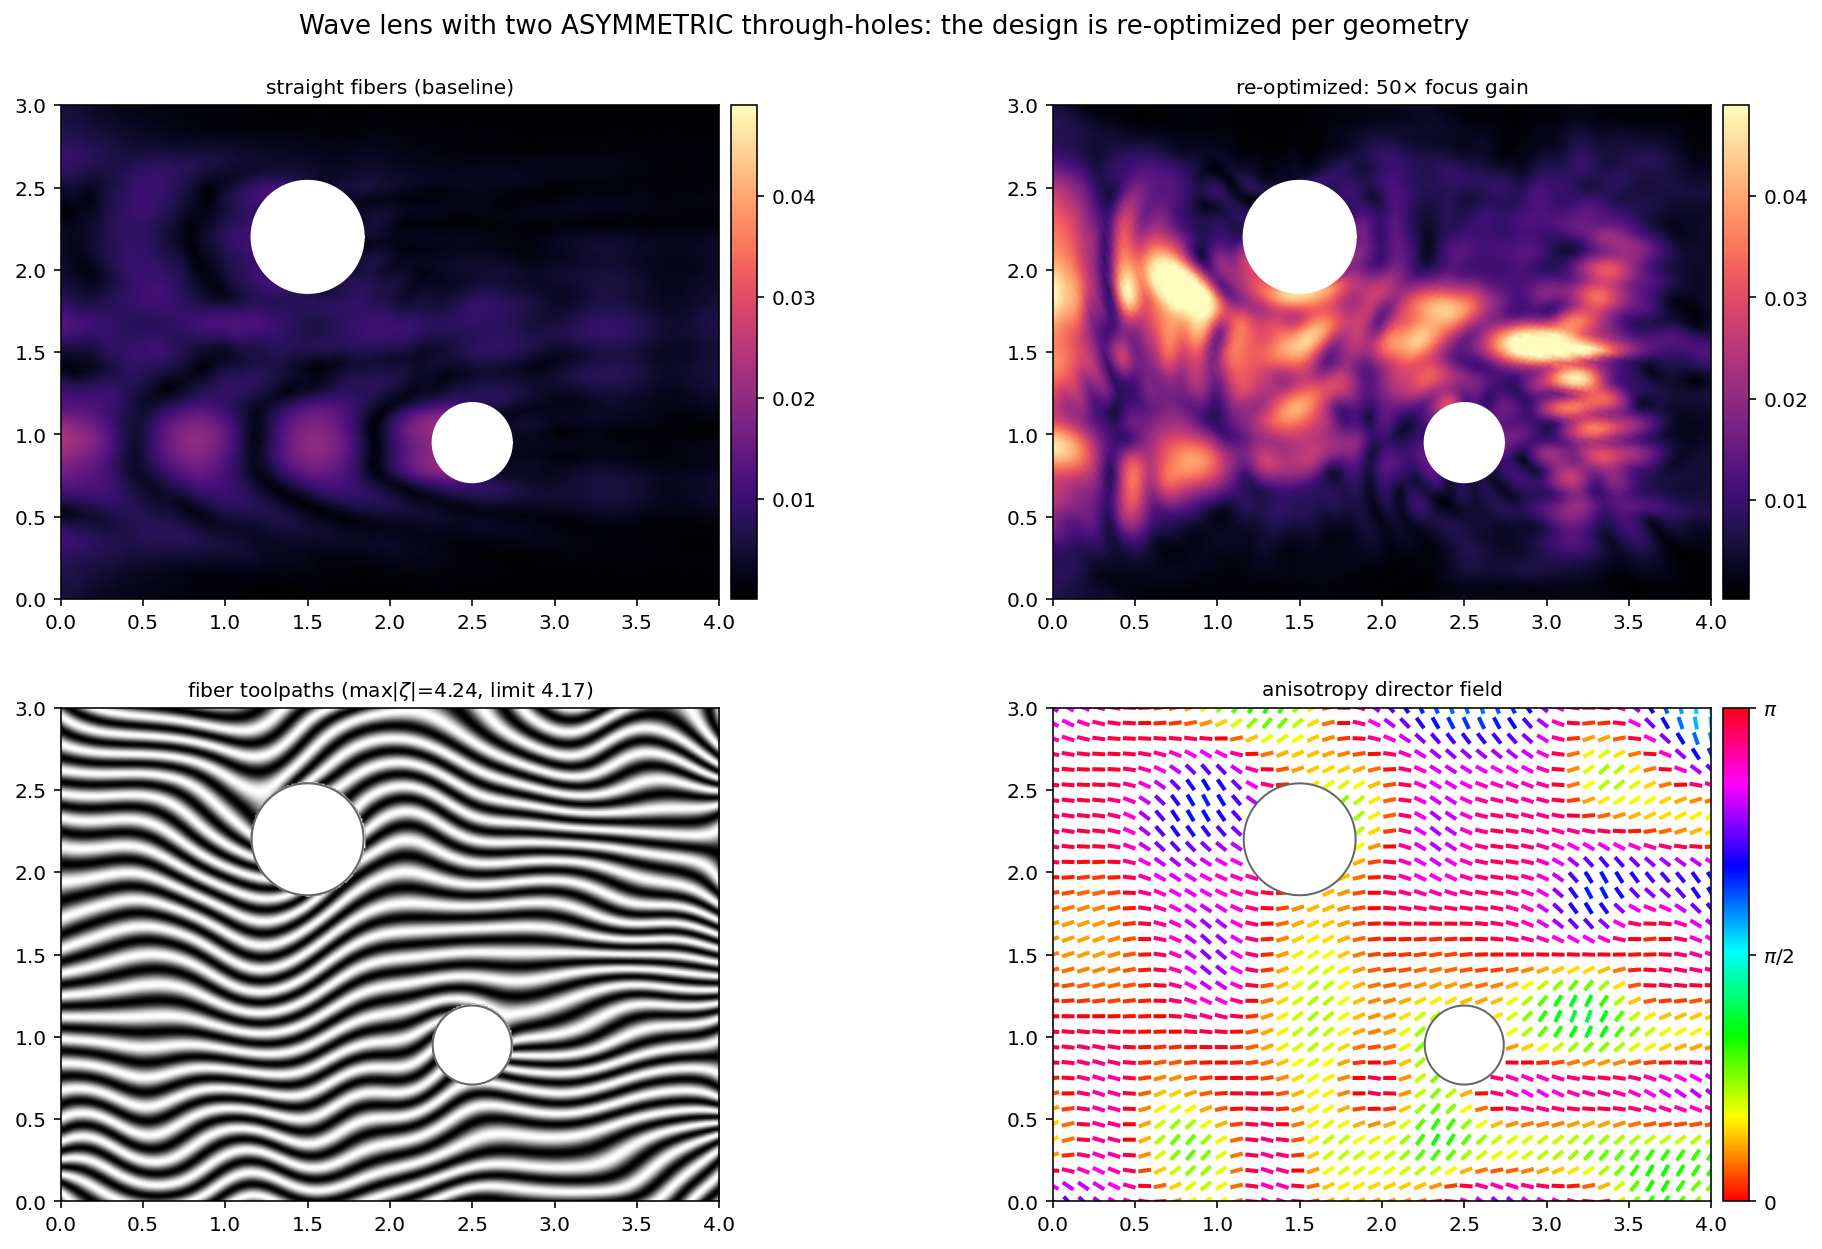
\includegraphics[width=0.74\textwidth]{dfx_lens_hole_asym.png}\\
\small Asymmetric holes, symmetry constraint dropped: $\AGAIN\times$.
\alert{Caveat:} converges to $|\zeta|_{\max}=\ACURL$ against a limit of $\ALIM$
--- a $1.7\%$ overshoot. The penalty is smooth, not a hard constraint.
\end{frame}

\begin{frame}{Elastic cloak of a conforming void}
\centering
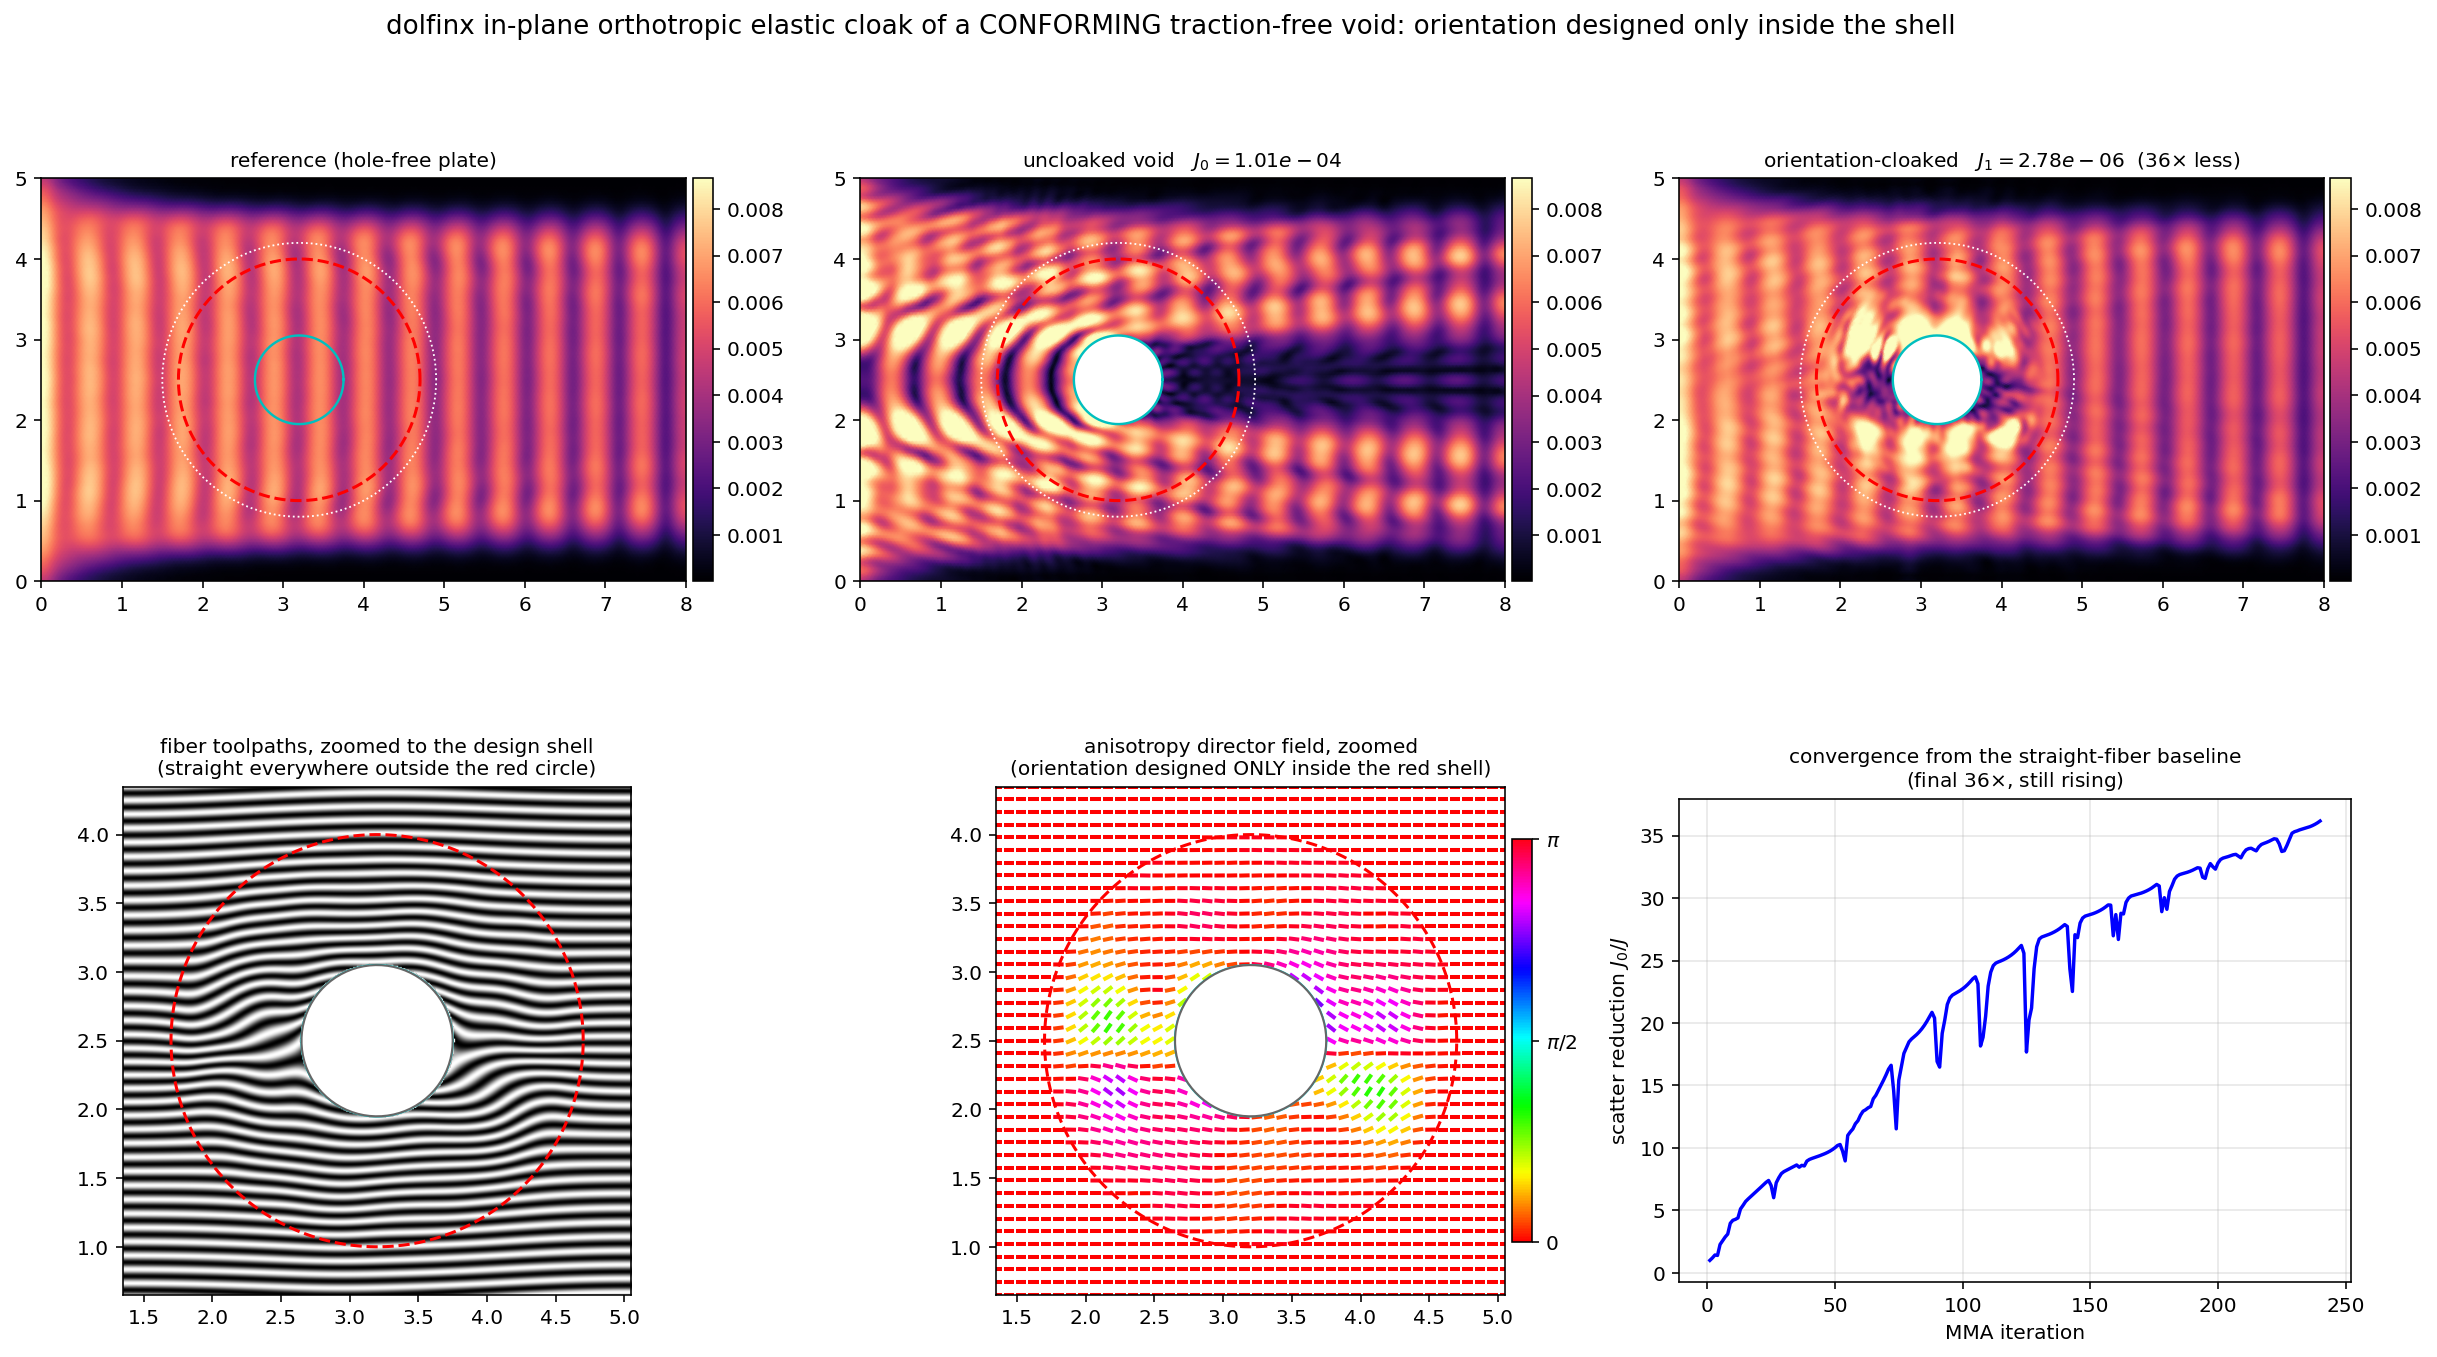
\includegraphics[width=0.80\textwidth]{dfx_cloak_conf.png}\\
\small Orientation designed \emph{only} inside the red shell (verified
$\max|\theta|=0$ outside): $\mathbf{36\times}$ scatter reduction, still rising at
240 iterations. Soft-void posing of the same problem gives markedly less.
\end{frame}

\begin{frame}{Routing energy around a joint}
\centering
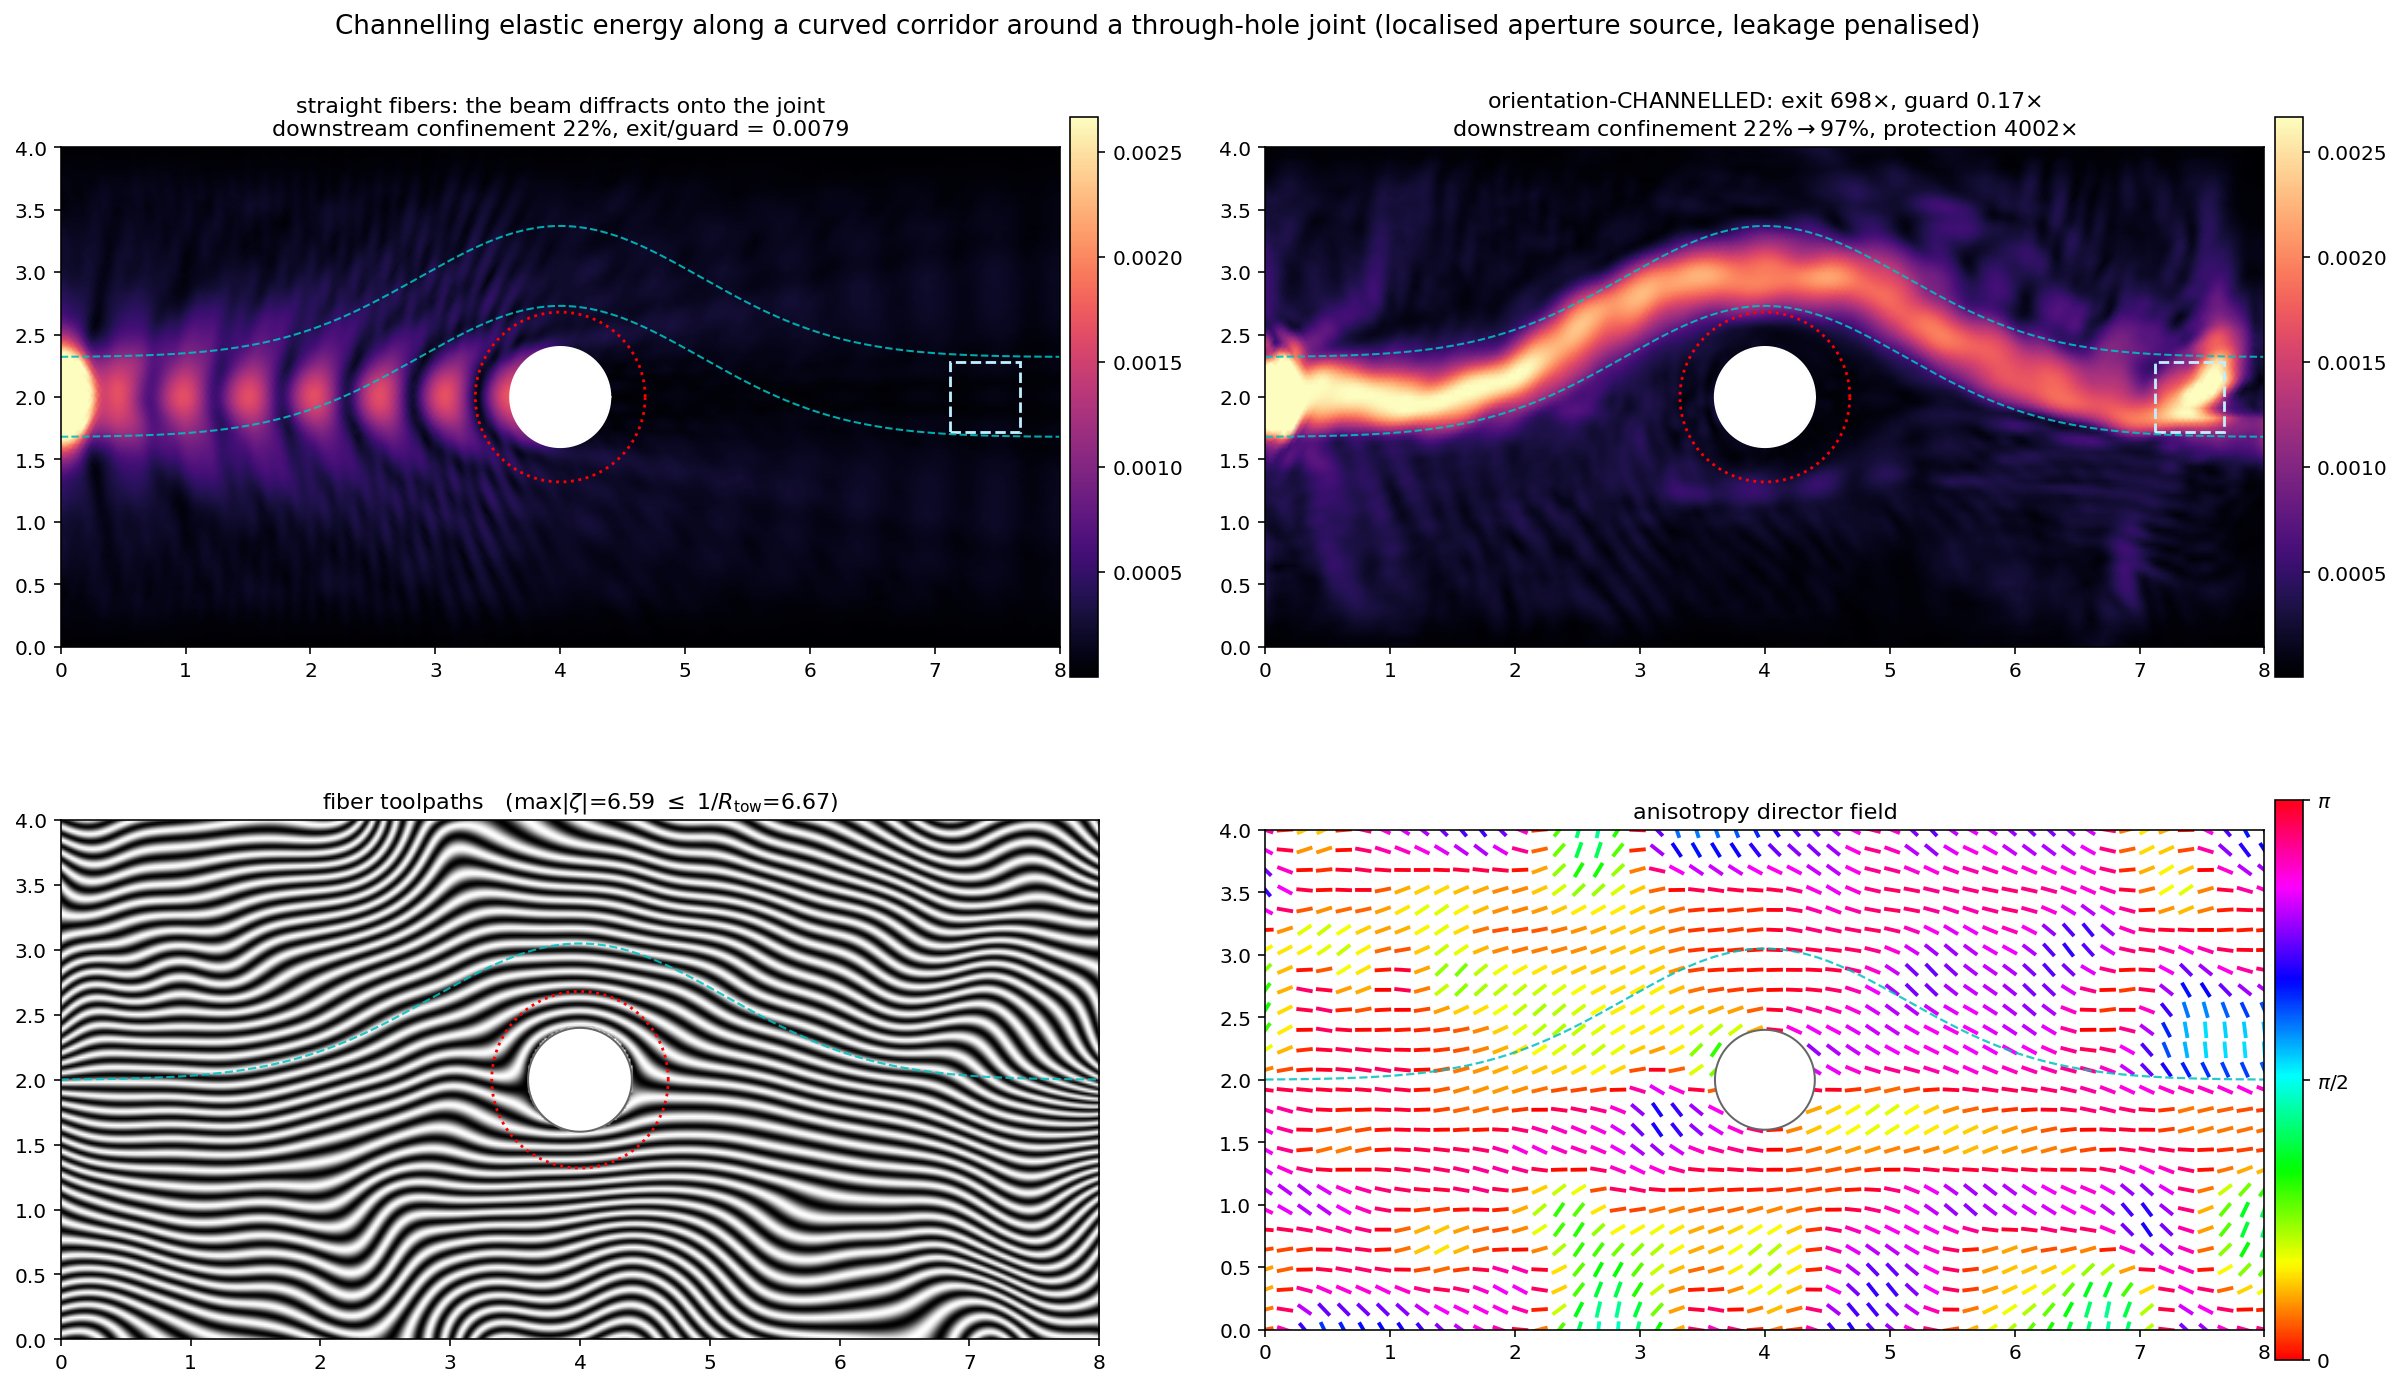
\includegraphics[width=0.72\textwidth]{dfx_guide_joint.png}\\
\small Exit $\GEXIT\times$, guard energy $\GGUARD$ of baseline, downstream
confinement $\GCONFZ\%\to\GCONFO\%$, feasible at $|\zeta|_{\max}=\GZ\le\GZALL$.
\end{frame}

\begin{frame}{What made the routing problem work}
Three modelling choices, each found by a \emph{silent} failure:
\begin{enumerate}
  \item \textbf{Localized source.} A plane wave leaves most of the field outside
        the corridor --- nothing to channel.
  \item \textbf{Print-head curvature limit, not the hole's.} $1/R_J$ is the rule
        for tows \emph{wrapping} a void; imposing it here pinned the design at
        the bound with the objective still negative.
  \item \textbf{Saturating delivery reward.} Linear in $E_{\rm exit}$, the
        delivered energy reached $6300\times$ and outweighed the guard penalty
        $760\!:\!1$ --- the optimizer bought delivery by making the joint
        $20\times$ \emph{busier}. A $\log$ reward fixes it.
\end{enumerate}
\vfill
\begin{alertblock}{All three returned healthy headline numbers}
They were caught by looking at the \emph{field} and the \emph{director map},
not the metric.
\end{alertblock}
\end{frame}

% ======================================================================== %
\section{Periodic metamaterials}

\begin{frame}{Flat band by co-designed topology and toolpath}
\[
  \mathbf K_r(\mathbf k)\bm\phi_n=\omega_n^2\mathbf M_r(\mathbf k)\bm\phi_n,
  \qquad \mathbf K_r=\mathbf T\HH\mathbf K\mathbf T
\]
\[
  J=w_{\rm f}\bigl(\widetilde{\max}_k\omega_b-\widetilde{\min}_k\omega_b\bigr)
   -w_{\uparrow}\text{(gap above)}-w_{\downarrow}\text{(gap below)}+c_v(\bar z-v^\star)^2
\]
\centering
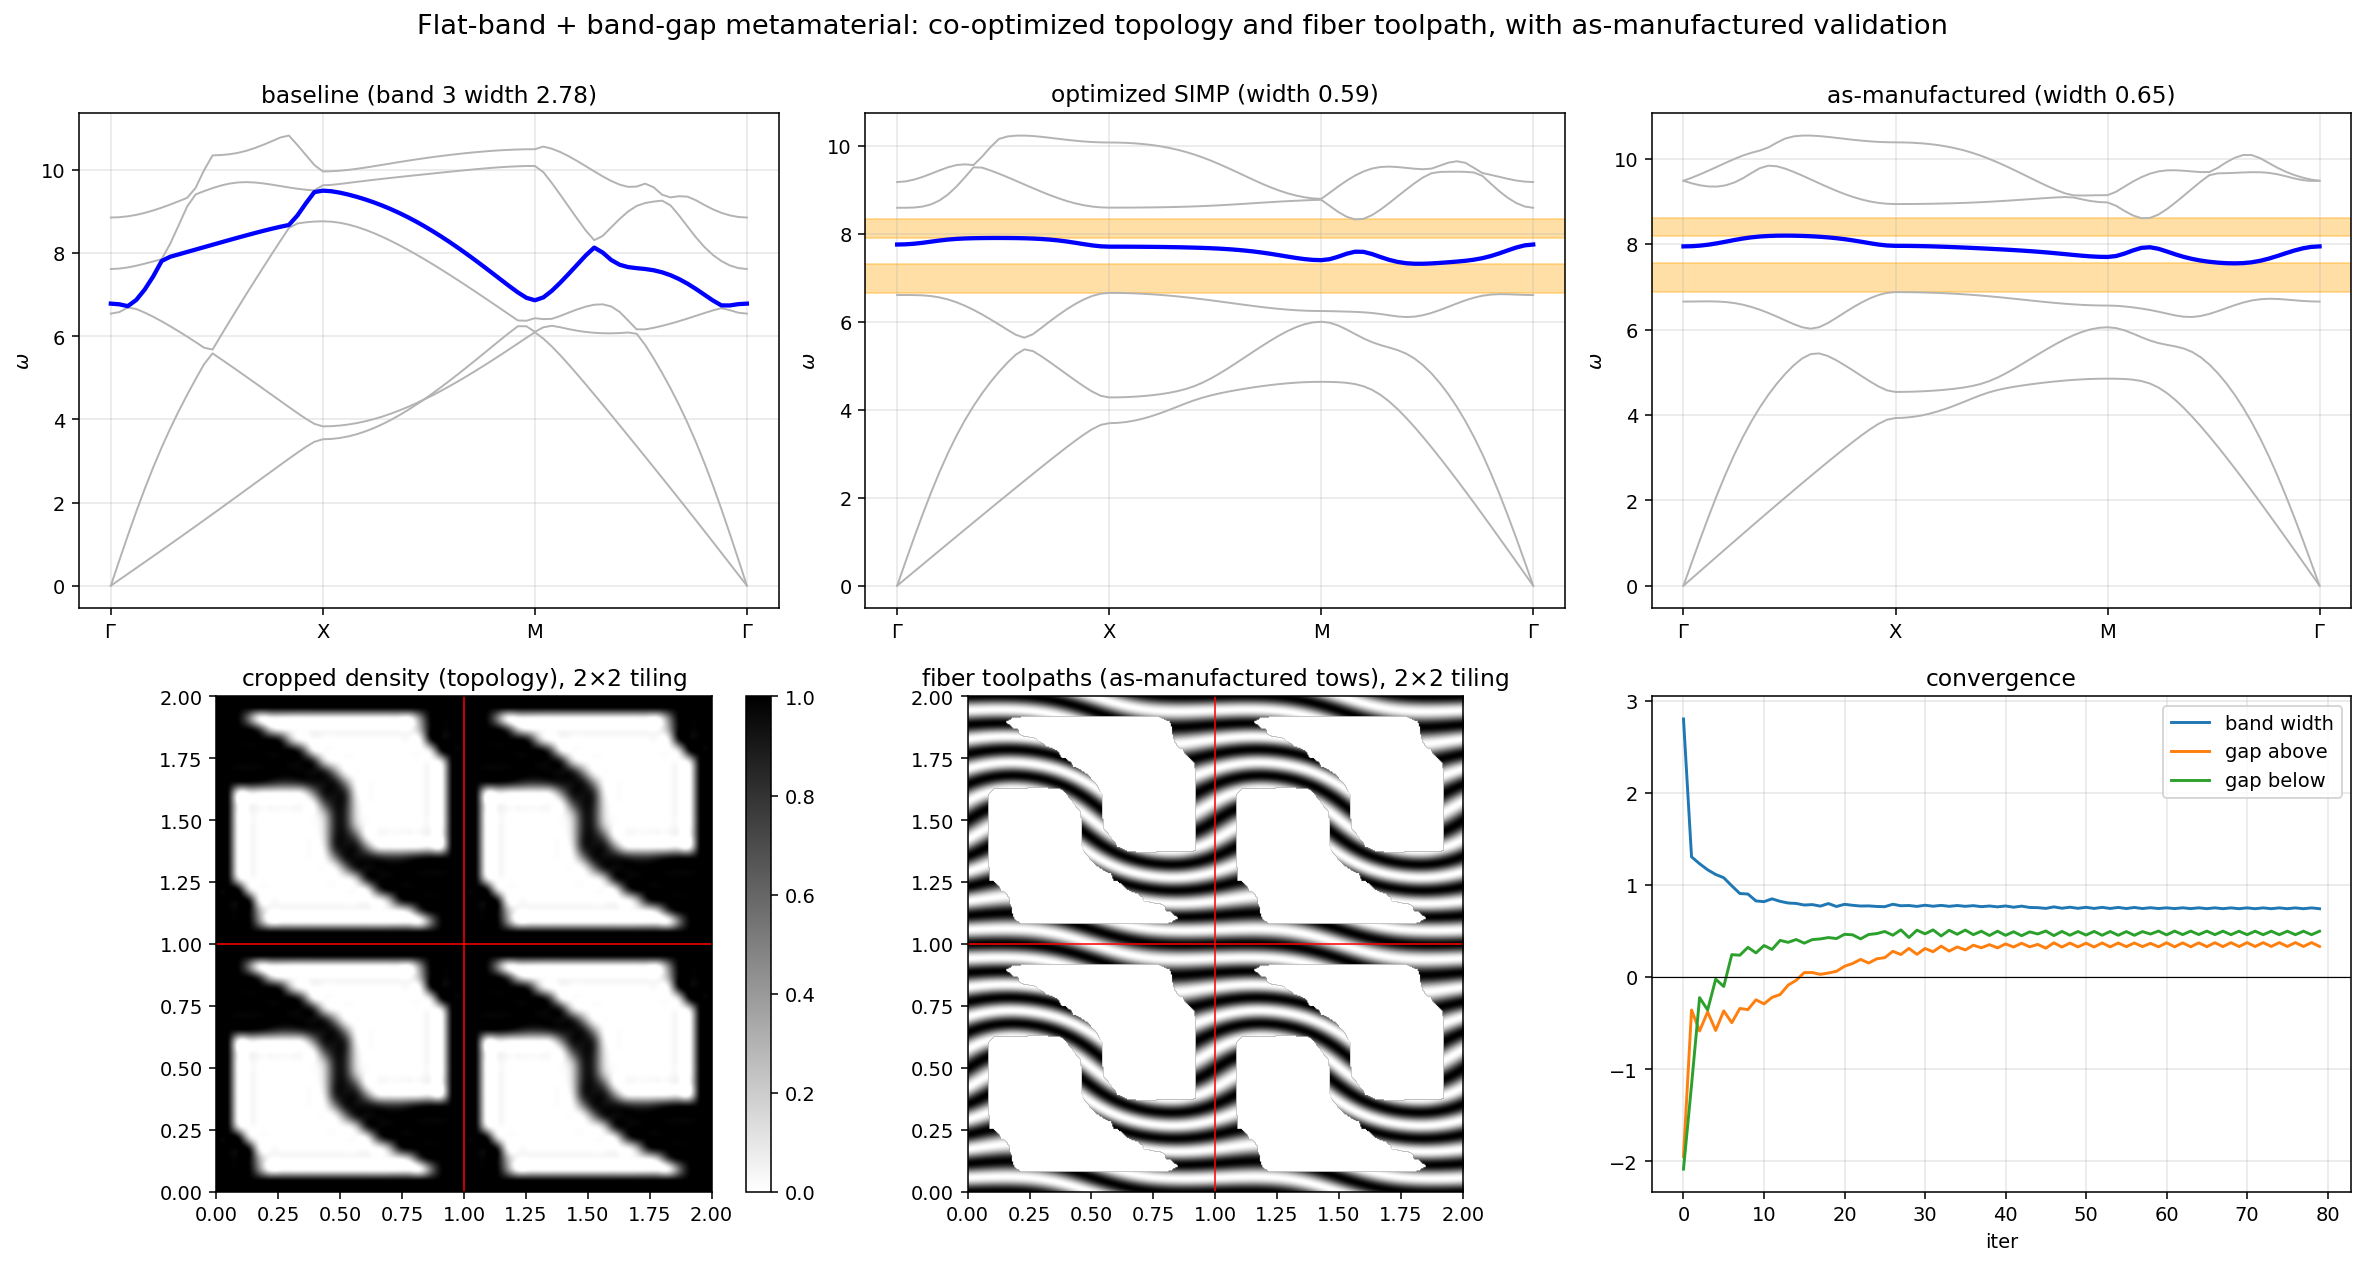
\includegraphics[width=0.66\textwidth]{flatband.png}\\
\small Band $\FBBAND$: width $\FBWZ\to\FBWO$, gaps $\FBGU$/$\FBGD$; survives the
as-manufactured crop ($\FBWV$, $\FBGUV$/$\FBGDV$).
\end{frame}

\begin{frame}{Does more design freedom help?}
\centering
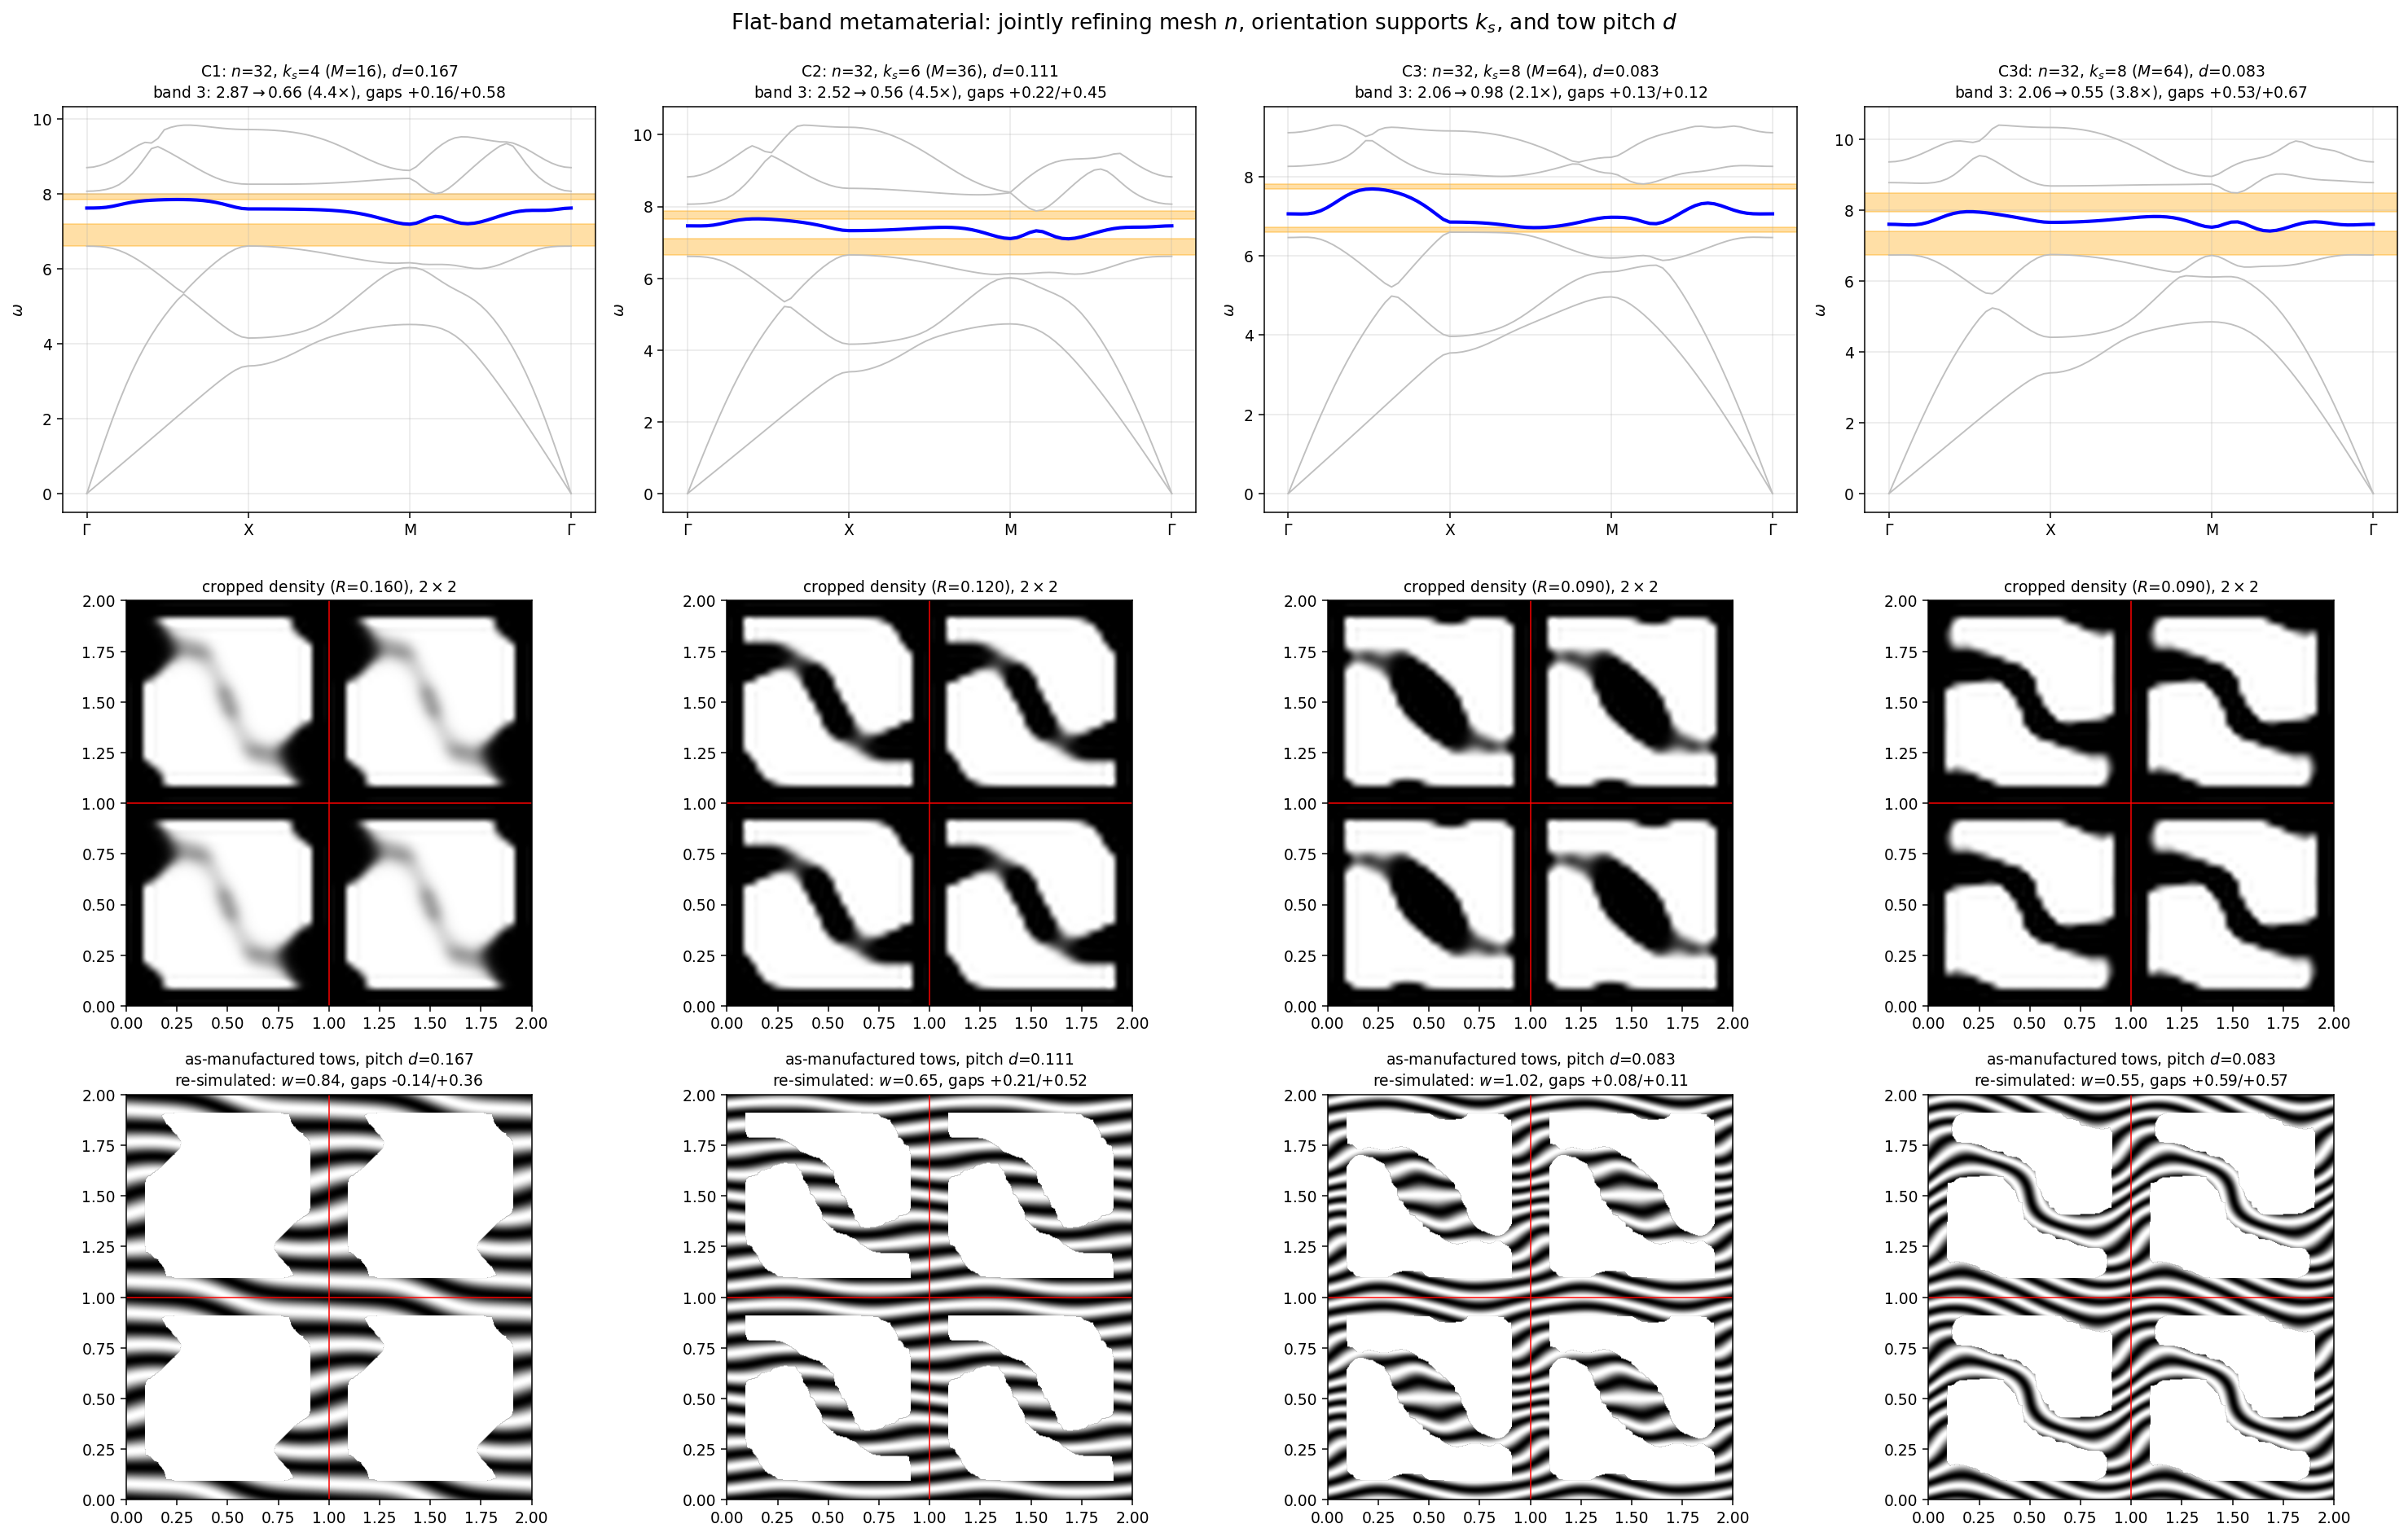
\includegraphics[width=0.99\textwidth]{flatband_sweep.png}
\end{frame}

\begin{frame}{Yes --- but only if the $\mathbf k$-sampling keeps up}
\centering\small
\begin{tabular}{lccccc}
\toprule
run & $k_s$ ($M$) & $N_k$ & $w_1$ (fine path) & $g_\uparrow$ & $g_\downarrow$\\
\midrule
C1  & 4 (16) & 22 & 0.66 & $+0.16$ & $+0.58$\\
C2  & 6 (36) & 22 & 0.56 & $+0.22$ & $+0.45$\\
C3  & 8 (64) & 22 & \alert{0.98} & $+0.13$ & $+0.12$\\
\textbf{C3d} & \textbf{8 (64)} & \textbf{40} & \textbf{0.55} & $\mathbf{+0.53}$ & $\mathbf{+0.67}$\\
\bottomrule
\end{tabular}
\vfill
\begin{block}{A free overfitting diagnostic}
KS aggregation can only \emph{over}-estimate a maximum. So if the width measured
on a fine path \emph{exceeds} the aggregate, the band is excursing between
samples. Aggregates: $0.79,\,0.70,\,0.67,\,0.68$ against fine
$0.66,\,0.56,\,\mathbf{0.98},\,0.55$ --- only C3, and C3 is the row that fails.
\end{block}
\end{frame}

% ======================================================================== %
\section{Closing}

\begin{frame}{What the optimizer taught us}
\begin{itemize}
  \item \textbf{Dips in the convergence curve were the optimizer, not the physics.}
        A line scan is smooth; excess $J$ scales as (step)$^2$. The MMA had no
        globalization and a move limit $1.84\times$ the design magnitude.
        An adaptive trust region: $23.5\times\to39.6\times$, zero dips.
  \item \textbf{Conforming meshes matter.} A staircased soft-void rim scatters on
        its own account; a large part of what the soft-void cloak cancelled was
        an artefact of the mesh.
  \item \textbf{Region specification is where the bugs hide.} Overlapping reward
        and penalty; rewarding accumulation instead of transport. Both returned
        confident numbers for designs doing the wrong thing.
  \item \textbf{MUMPS over PETSc's built-in LU: $4.4\times$}, identical answers.
\end{itemize}
\end{frame}

\begin{frame}{Summary}
Orientation-only design, one material, manufacturable toolpaths throughout:
\begin{center}\small
\begin{tabular}{ll}
\toprule
wave lens                       & $78\times$ focus gain\\
\quad under $|\zeta|\le\zeta_{\rm all}$ & $\GAINC\times$\\
through-holes (conforming)      & $\HGAINU\times$ / $\HGAINC\times$ constrained\\
asymmetric holes                & $\AGAIN\times$ (re-solved per geometry)\\
elastic cloak (shell-confined)  & $36\times$ scatter reduction\\
joint routing                   & $\GEXIT\times$ exit, guard $\GGUARD$, conf.\ $\GCONFO\%$\\
flat band                       & $\FBWZ\to\FBWO$, both gaps open\\
\bottomrule
\end{tabular}
\end{center}
\vfill
All of it rests on one exact statement: for an isotropic plate
$\partial\mathbf D_f/\partial\theta\equiv\bm 0$, so the identical code returns
\emph{exactly} the baseline. Anisotropy --- supplied physically by the
continuous-fiber toolpath --- is the necessary and sufficient mechanism.
\end{frame}

\end{document}
